\chapter{Case study}
This chapter presents a case study where the load forecasting system is applied to Bruny Island.
As discussed in section \ref{scope} (\nameref{scope}), the aim of this case study is to develop a load forecasting system which can predict future load based on weather, holiday periods, car movement, and other factors. 
Bruny Island and the NAC will be used as a case study. 
The forecasting system will be equally applicable to any power system network, \hl{and this will be demonstrated later in this chapter}.
\\
Specifically, the system will have the following properties:
\begin{itemize}
	\item The system will produce a forecast up to 24 hours in the future in 15- to 60-minute intervals. This will be a rolling forecast that can be re-calculated at any time.
	\item The forecast will be able to begin from any point time.
	\item The forecast will predict load in kVA at each interval.
	\item The forecast system will be aimed at predicting aggregate load at the feeder level. That is, between approximately 0.5 and 10MVA.
	\item The forecast system will be especially tuned to predict load during holiday periods.
\end{itemize}

\begin{figure}
	\centering
	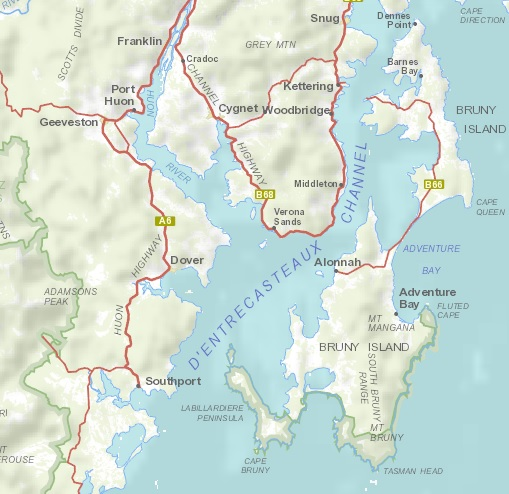
\includegraphics[width=0.35\linewidth]{images/bruny-basic}
	\caption{Bruny Island, in southern Tasmania, Australia. TODO: make a map that has expanded views to show the location on world map. QGIS, perhaps.}
	\label{fig:bruny-basic}
\end{figure}


\section{Data analysis}
\begin{itemize}
	\item \hl{this dot point list is for planning}
	\item discuss available data - load, weather, cars, other feeders and reclosers
	\item general load profiles of winter week, summer week, and full year
	\item look at annual growth of electricity. I need to investigate further my graph that is anomalous for 2013 and 2014 in growth.
	\item talk about different days of the week, and relate to car movement
	\item Look at special days - easter, june, christmas/ny
	\item talk about relationship between load and weather - temperature mainly
	\item Is load influenced by humidity like literature claims, or are temperature and humidity simply related?
	\item look at coloured scatter plot of load, temperature, and cumulative cars - more people correlates with more load in general - but we don't know future number of people.
	\item correlation matrix for power, cars, and weather
	\item cross correlations. Especially discuss any lags
	\item perhaps conclude with some important takeaways
	
\end{itemize}

In section \ref{patterns-profiles} the general properties of load profiles and how they are influenced by exogenous factors was discussed. Now, these general properties will be investigated in depth for the particular feeder in the case study.
\par
let's begin by having a simple look at some load profiles from the island.
Figure \ref{fig:load-profiles} shows apparent power draw on Bruny Island over a winter week, a summer week, and over an entire year.
The two weeks were selected to avoid special days such as holidays and are representative of typical weeks.
Some observations are immediately obvious
\begin{itemize}
	\item The midday load is only marginally larger than the overnight load in summer, but in winter it is significantly larger.
	\item Morning peaks are larger than afternoon peaks in summer, but in winter they are approximately equal.
	\item Thursday midday of the summer week appears abnormally high - perhaps this is a special day.
	\item There is some bad data on Tuesday of the summer week, as well as some missing data throughout the year.
	\item Over the whole year there appears to be a trend of increased max daily load over winter, which coincides with colder weather.
	\item There are some periods of abnormally large load over the year: March 27, June 11, and December 28.
\end{itemize}

\begin{figure}[htbp]
	\centering
	\subfigure[]{
		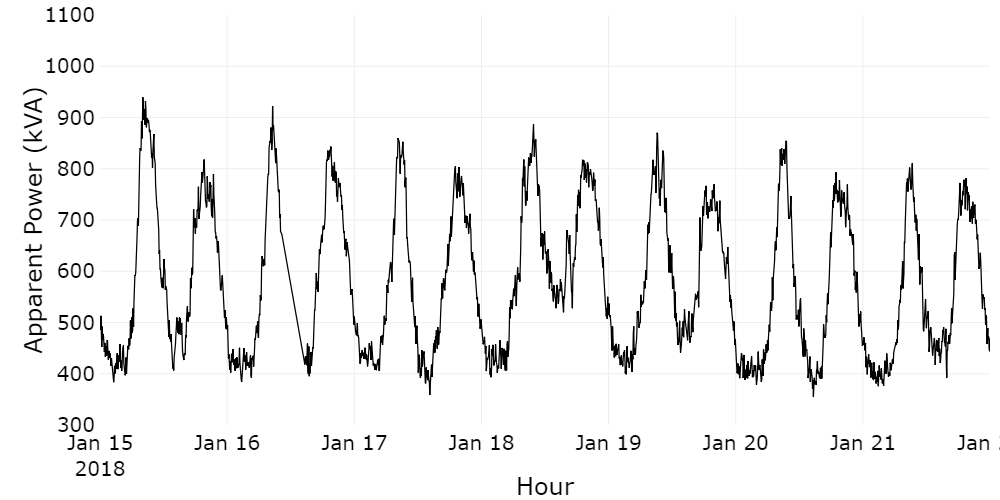
\includegraphics[width=.7\textwidth]{images/simple-week-summer}
		\label{fig:simple-week-summer}}
	\vfil
	\subfigure[]{
		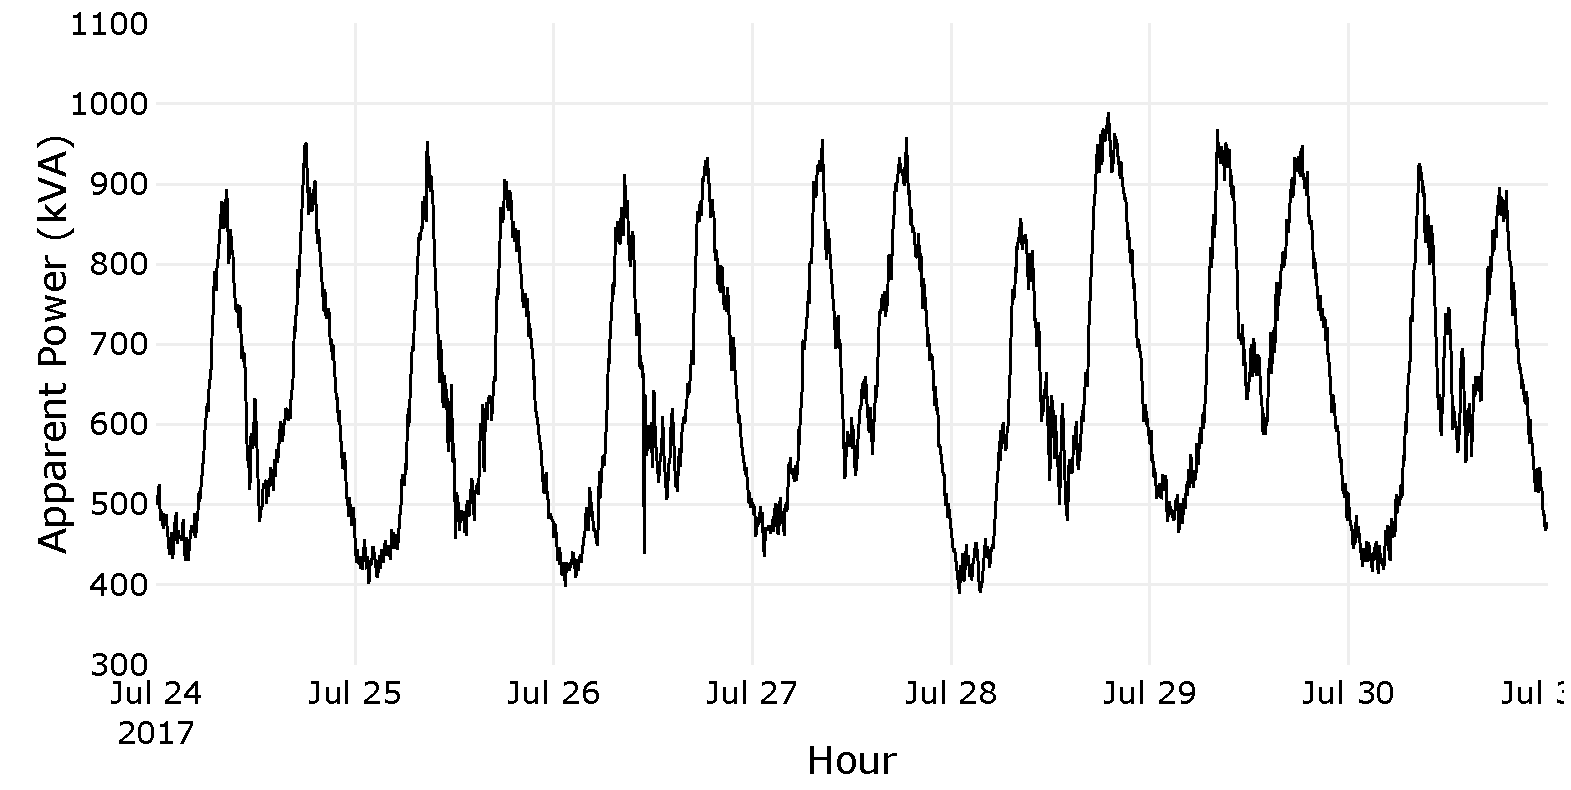
\includegraphics[width=.7\textwidth]{images/simple-week-winter}
		\label{fig:simple-week-winter}}
	\vfil
	\subfigure[]{
		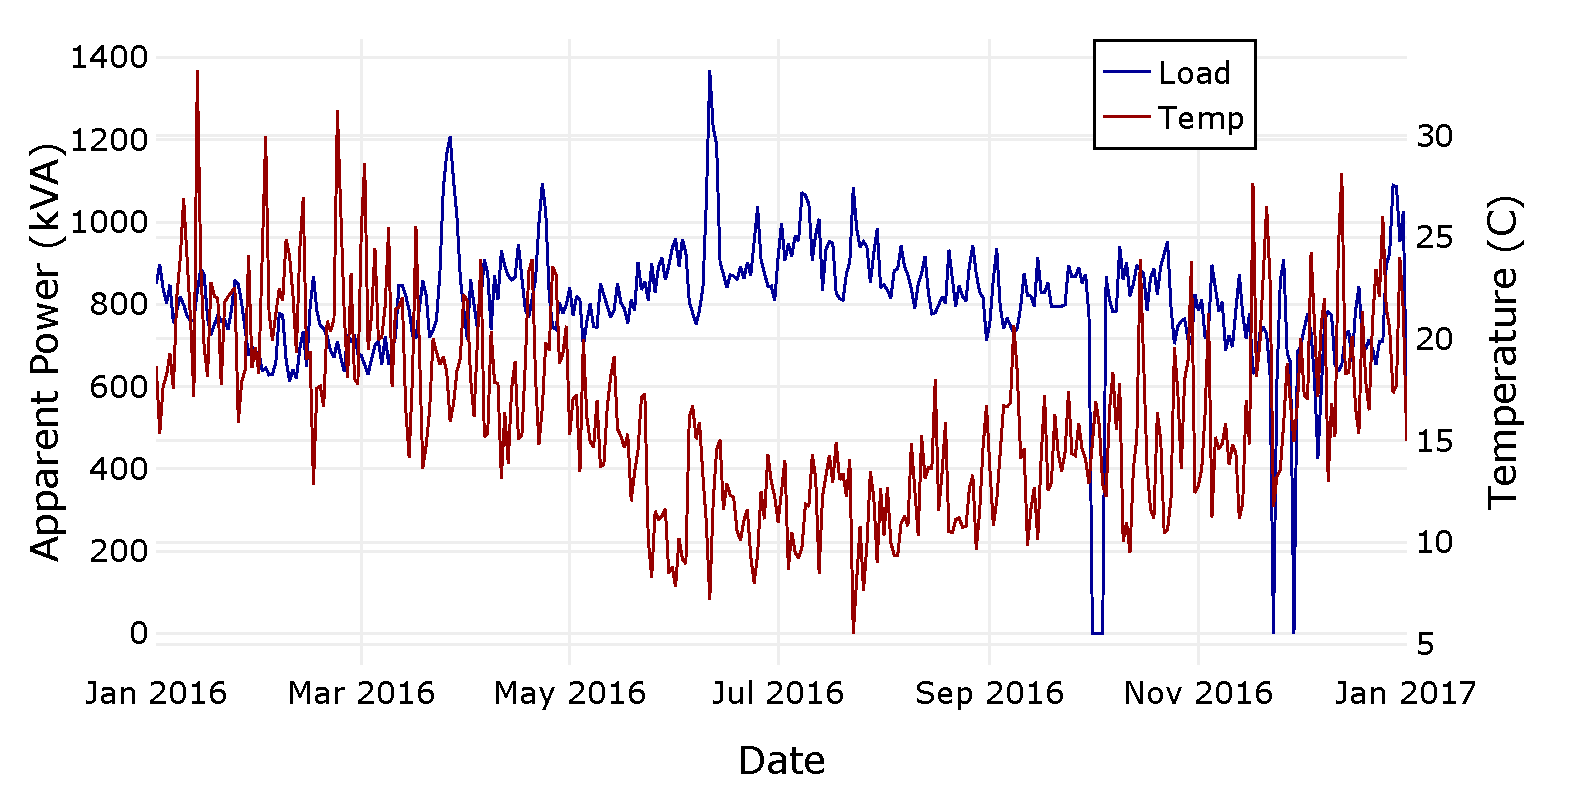
\includegraphics[width=.7\textwidth]{images/max-load-max-temp}
		\label{fig:max-load-max-temp}}
	\caption{Bruny Island load profiles. (a) Load over a single summer week in 2018. (b) Load over a single winter week in 2017. (c) Peak daily load and peak daily temperature over all of 2017.}
	\label{fig:load-profiles}
\end{figure}

It was mentioned in section \ref{pattens-profiles} that weekends and weekdays tend to have different load profiles, but this is not immediately obvious from figure \ref{fig:load-profiles}.
Figure \ref{fig:average-profiles} shows this difference between days of the week.
What is immediately obviously is that the differences between days of the week are not restricted to 24 hour bounds - the different load profile shapes gently merge into each other over the course of an afternoon or morning.
% This is an especially important observation for a forecasting system that needs to be able to perform forecasts not just at a single time each day, but at any time.
It can be seen that the Friday profile morphs into the Saturday profile during the afternoon, perhaps as people arrive on the island for the weekend, and the Sunday profile morphs into a weekday profile over the afternoon, perhaps as people depart the island.
\par
Figures \ref{fig:average-arriving} and \ref{fig:average-departing} further support that the changes in load profiles are a result of people arriving on or leaving the island.
It can be seen that many cars tend to arrive on the island on Friday afternoon, leading to the change in load profile between Friday and Saturday.
Likewise, many cars leave the island on Sunday afternoon, shifting the load profile from Sunday to a weekday.
\begin{figure}[htbp]
	\centering
	\subfigure[]{
		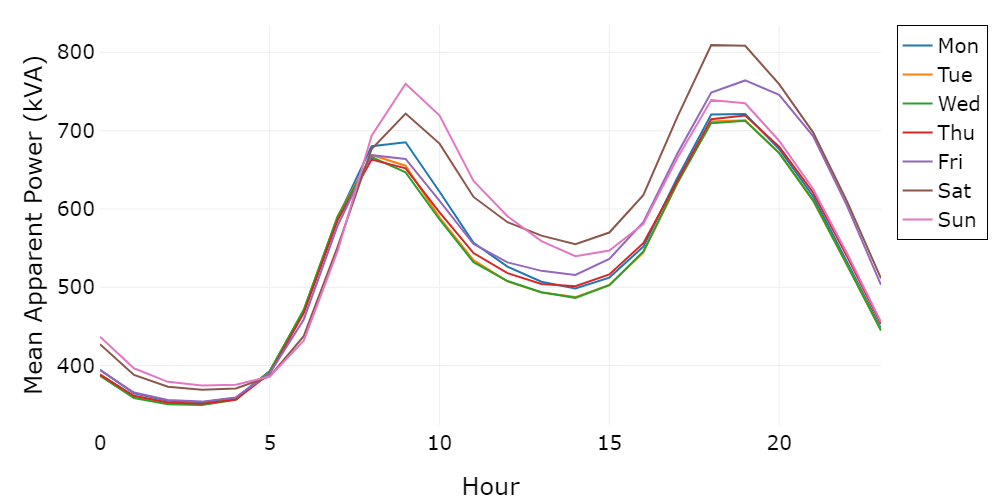
\includegraphics[width=.7\textwidth]{images/average-profiles}
		\label{fig:average-profiles}}
	\vfil
	\subfigure[]{
		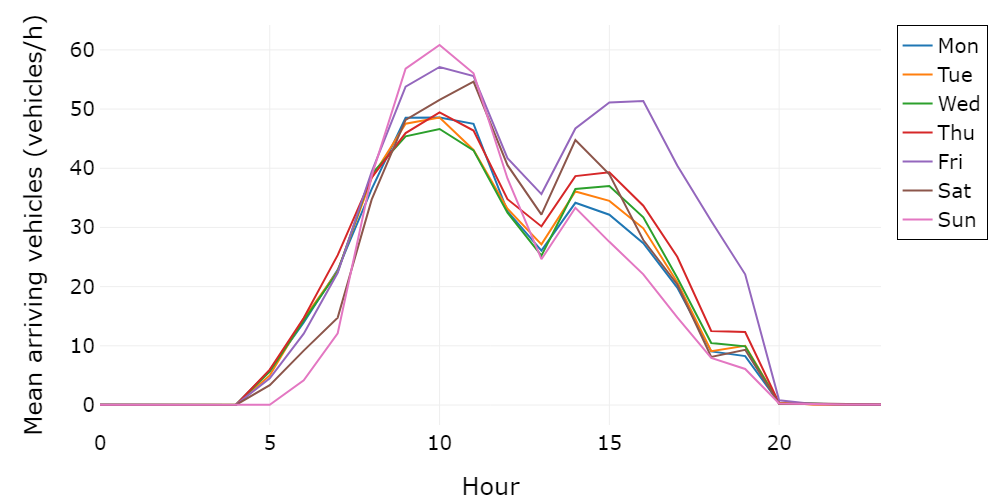
\includegraphics[width=.7\textwidth]{images/average-arriving}
		\label{fig:average-arriving}}
	\vfil
	\subfigure[]{
		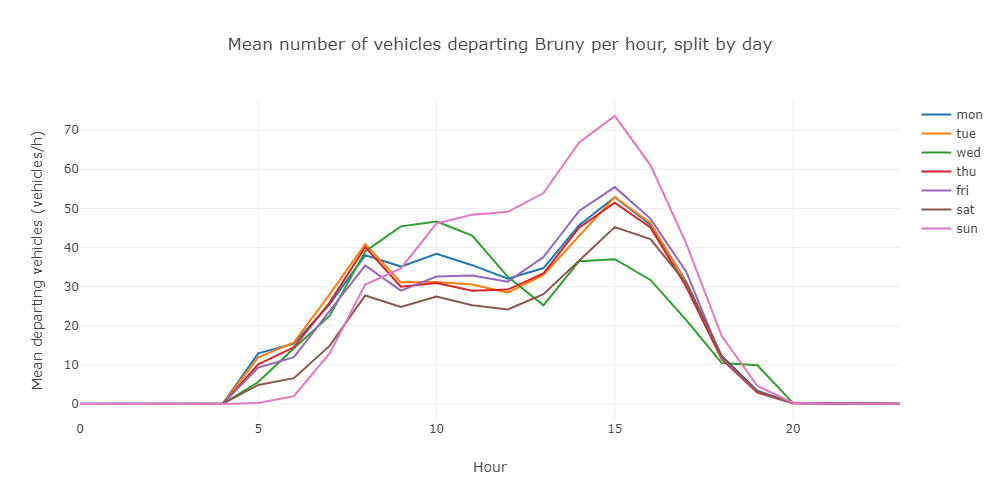
\includegraphics[width=.7\textwidth]{images/average-departing}
		\label{fig:average-departing}}
	\caption{Bruny Island average load profiles. (a) Average load profiles for each day of the week. Average number of cars arriving on (b) and leaving (c) the island each day.}
	\label{fig:average-load-profiles}
\end{figure}

\subsection{Forecasting system architecture}
\begin{itemize}
	\item Transformer at core
	\item set of input vectors
	\item handling of bad data
	\item similar day selection
	\item 
\end{itemize}